\documentclass[compress,red]{beamer}
\usepackage{etex}
\mode<presentation>

\usepackage{amsmath}
\usepackage{amsthm}

%%%%%%%%%%%%%%%%%%%%%%%%%%%%%%%%%%%%%%%%
                                       %
% change this line for portable code:  %
\newcommand*{\commonDir}{../../common/}%
\input{\commonDir preambleCommon}      %
                                       %
%%%%%%%%%%%%%%%%%%%%%%%%%%%%%%%%%%%%%%%%

\graphicspath{{../../falconBioinfo/figures/}{./figures}}

\usetheme{Warsaw}
% other themes: AnnArbor, Antibes, Bergen, Berkeley, Berlin, Boadilla, boxes, CambridgeUS, Copenhagen, Darmstadt, default, Dresden, Frankfurt, Goettingen,
% Hannover, Ilmenau, JuanLesPins, Luebeck, Madrid, Maloe, Marburg, Montpellier, PaloAlto, Pittsburg, Rochester, Singapore, Szeged, classic

%\usecolortheme{lily}
% color themes: albatross, beaver, beetle, crane, default, dolphin, dov, fly, lily, orchid, rose, seagull, seahorse, sidebartab, structure, whale, wolverine

%\usefonttheme{serif}
% font themes: default, professionalfonts, serif, structurebold, structureitalicserif, structuresmallcapsserif

\hypersetup{pdfpagemode=FullScreen} % makes your presentation go automatically to full screen

% define your own colors:
\definecolor{CURed}{rgb}{0.702,0.106,0.106}
\definecolor{CUGrey}{rgb}{0.302,0.31,0.3255}
%
\definecolor{White}{rgb}{1,1,1}
\definecolor{Red}{rgb}{1,0,0}
\definecolor{Blue}{rgb}{0,0,1}
\definecolor{Green}{rgb}{0,1,0}
\definecolor{magenta}{rgb}{1,0,.6}
\definecolor{lightblue}{rgb}{0,.5,1}
\definecolor{lightpurple}{rgb}{.6,.4,1}
\definecolor{gold}{rgb}{.6,.5,0}
\definecolor{orange}{rgb}{1,0.4,0}
\definecolor{hotpink}{rgb}{1,0,0.5}
\definecolor{newcolor2}{rgb}{.5,.3,.5}
\definecolor{newcolor}{rgb}{0,.3,1}
\definecolor{newcolor3}{rgb}{1,0,.35}
\definecolor{darkgreen1}{rgb}{0, .35, 0}
\definecolor{darkgreen}{rgb}{0, .6, 0}
\definecolor{darkred}{rgb}{.75,0,0}

\xdefinecolor{olive}{cmyk}{0.64,0,0.95,0.4}
\xdefinecolor{purpleish}{cmyk}{0.75,0.75,0,0}

% can also choose different themes for the "inside" and "outside"

% \usepackage{beamerinnertheme_______}
% inner themes include circles, default, inmargin, rectangles, rounded

% \usepackage{beamerouterthemesmoothbars}
% outer themes include default, infolines, miniframes, shadow, sidebar, smoothbars, smoothtree, split, tree

\useoutertheme[subsection=false]{smoothbars}

% to have the same footer on all slides
%\setbeamertemplate{footline}[text line]{STUFF HERE!}
\setbeamertemplate{footline}[text line]{} % makes the footer EMPTY

% Change some colors:
\setbeamercolor{structure}{fg=CURed}
\setbeamercolor*{palette quaternary}{fg=white,bg=CUGrey}

% include packages
\usepackage{multicol}
\usepackage{epsfig}
\usepackage[all,knot]{xy}
\xyoption{arc}
\usepackage{url}
\usepackage{multimedia}
\usepackage{hyperref}
     
%%%%%%%%%%%%%%%%%%%%%%%%%%%%%%%%%%%%%%%%%%%%%%%%%%%%%%%%%%%%%%%%%%%%%%%%%%%%%%%%%%%%%%%%%%
%%%%%%%%%%%%%%%%%%%%%%%%%%%%%% Title Page Info %%%%%%%%%%%%%%%%%%%%%%%%%%%%%%%%%%%%%%%%%%%
%%%%%%%%%%%%%%%%%%%%%%%%%%%%%%%%%%%%%%%%%%%%%%%%%%%%%%%%%%%%%%%%%%%%%%%%%%%%%%%%%%%%%%%%%%

\title{Estimating Metabolic Fluxes from Gene Expression}
\subtitle{A Principled and Efficient Approach}
\author{\texorpdfstring{Brandon Barker\newline
  \url{brandon.barker@gmail.com}}{Brandon Barker}}
\institute{
Tri-Institutional Program in Computational Biology and Medicine\\ 
Gu Laboratory\\
Cornell University \\ \vspace{.25cm}CAC Job Search}
\date{\today}

%%%%%%%%%%%%%%%%%%%%%%%%%%%%%%%%%%%%%%%%%%%%%%%%%%%%%%%%%%%%%%%%%%%%%%%%%%%%%%%%%%%%%%%%%%
%%%%%%%%%%%%%%%%%%%%%%%%%%%%%% Begin Your Document %%%%%%%%%%%%%%%%%%%%%%%%%%%%%%%%%%%%%%%
%%%%%%%%%%%%%%%%%%%%%%%%%%%%%%%%%%%%%%%%%%%%%%%%%%%%%%%%%%%%%%%%%%%%%%%%%%%%%%%%%%%%%%%%%%

\begin{document}


%%%%%%%%%%%%%%%%%%%%%%%%%%%%%%%%%%%%%%%%
                                       %
\newboolean{thesisStyle}               %
\setboolean{thesisStyle}{true}         %
                                       %
\input{\commonDir documentHeadCommon}  %
                                       %
%%%%%%%%%%%%%%%%%%%%%%%%%%%%%%%%%%%%%%%%

%%%%%%%%%%%%%%%%%%%%%%%%%%%%%%%%%%%%%%%%%%%%%%%%%%%%%%%%%%%%%%%%%%%%%%%%%%%%%%%%%%%%%%%%%%

\frame{
	\titlepage 
}

%%%%%%%%%%%%%%%%%%%%%%%%%%%%%%%%%%%%%%%%%%%%%%%%%%%%%%%%%%%%%%%%%%%%%%%%%%%%%%%%%%%%%%%%%%
% this puts the outline before EACH section automatically & will
% highlight the section you're about to talk about
%\section[Outline]{}
%\frame{\tableofcontents}

%%%%%%%%%%%%%%%%%%%%%%%%%%%%%%%%%%%%%%%%%%%%%%%%%%%%%%%%%%%%%%%%%%%%%%%%%%%%%%%%%%%%%%%%%%

\section{Introduction}
\subsection{Beamer Intro}

%%%%%%%%%%%%%%%%%%%%%%%%%%%%%%%%%%%%%%%%%%%%%%%%%%%%%%%%%%%%%%%%%%%%%%%%%%%%%%%%%%%%%%%%%%

\frame{\frametitle{}
\begin{center}
\begin{block}<+->{Disclaimer \#1}
	\vspace{.1cm}
	\begin{center} \large
	I am \textcolor{darkgreen}{NOT} an expert in \LaTeX\\ \vspace{.1cm}
	I am \textcolor{darkgreen}{NOT} an expert in Beamer\\
	\end{center}
\end{block}
\vspace{1cm}
\begin{block}{Disclaimer \#2}
	\vspace{.1cm}
	This talk is designed to \textcolor{darkgreen}{introduce} you to presentations in \LaTeX\\ \vspace{.1cm}
	\begin{center}
	$\dots$ and showcase cool features of Beamer\\
	\end{center}
\end{block}
\end{center}
}

%%%%%%%%%%%%%%%%%%%%%%%%%%%%%%%%%%%%%%%%%%%%%%%%%%%%%%%%%%%%%%%%%%%%%%%%%%%%%%%%%%%%%%%%%%

\frame{\frametitle{}

\begin{figure}
\centering
\begin{tikzpicture}[scale=0.5, every node/.style={scale=0.5}]%[scale=0.8, node distance = 1cm, auto]
    % Place nodes
    \node [block] (start) {start}; 
    \node [iogram, below of=start, left of=start, xshift=-0.2cm] (exp) {Genes:\\ expression 
      ($\mu$,~$\sigma$)}; 
    \node [iogram, below of=start, right of=start] (rules) {Reactions:
      GPR Rule}; 
    \node [block, below of=rules] (parse) {Parse Rule}; 
    \node [block, below of=parse, left of=parse, xshift=-0.5cm]
      (mindisj) {Find minimum disjunction};
    \node [iogram, below of=mindisj] (expstd)
          {Reactions (enzyme~complexes):\\ abundance ($\mu$,~$\sigma$)};
    \node [iogram, right of=falcon, below of=expstd, xshift=0.2cm] (smat) 
      {$\mathbf{S}$ matrix};
    \node [iogram, left of=falcon, below of=expstd, xshift=-0.3cm] (vbnd) 
      {Reactions:\\ flux bounds ($\mathbf{v}_{lb}$, $\mathbf{v}_{ub}$)};
    \node [block, below of=vbnd, left of=smat, right of=vbnd, 
      below of=expstd, yshift=-0.5cm] (falcon) 
      {Flux fitting (FALCON)};
    \node [iogram, below of=falcon] (fluxout) 
      {Reactions:\\ fluxes ($\mathbf{v}:$ $\mu$,~$\sigma$)};
    % Draw edges
    \path [line] (start) -- (exp);
    \path [line] (start) -- (rules);
    \path [line] (rules) -- (parse);
    \path [line] (exp.south) -- (mindisj);
    \path [line] (parse) -- (mindisj);
    \path [line] (mindisj) -- (expstd);
    \path [line, transform canvas={xshift=0.1cm}] (expstd) -- (falcon);
    \path [line] (rules.east) |- (falcon.east);
    \path [line] (smat) -- (falcon);
    \path [line] (vbnd) -- (falcon);
    \path [line] (falcon) -- (fluxout);

\end{tikzpicture}
\caption{Flowchart illustrating the two algorithms in the pipeline.}
\end{figure}

}

%%%%%%%%%%%%%%%%%%%%%%%%%%%%%%%%%%%%%%%%%%%%%%%%%%%%%%%%%%%%%%%%%%%%%%%%%%%%%%%%%%%%%%%%%%

\frame{\frametitle{Equivalent GPR rules can be evaluated differently}

\begin{center}
\begin{tabular}{cccccccc}
$r_1$ & := & [A and B] or [A and C] & $\rightarrow$ & $e_1$  &=& $\min(a,b$) + $\min(a,c$) \\ 
$r_2$ & := & [A and (B or C)]       & $\rightarrow$ & $e_2$  &=&  $\min(a, b + c$) 
\end{tabular} 
\end{center}

}
%%%%%%%%%%%%%%%%%%%%%%%%%%%%%%%%%%%%%%%%%%%%%%%%%%%%%%%%%%%%%%%%%%%%%%%%%%%%%%%%%%%%%%%%%%

\frame{\frametitle{Grouping reactions by enzyme complex has a large effect} 

\begin{figure}
\centering
\begin{tabular}{cc}
  \begin{subfigure}[b]{0.45\textwidth}
  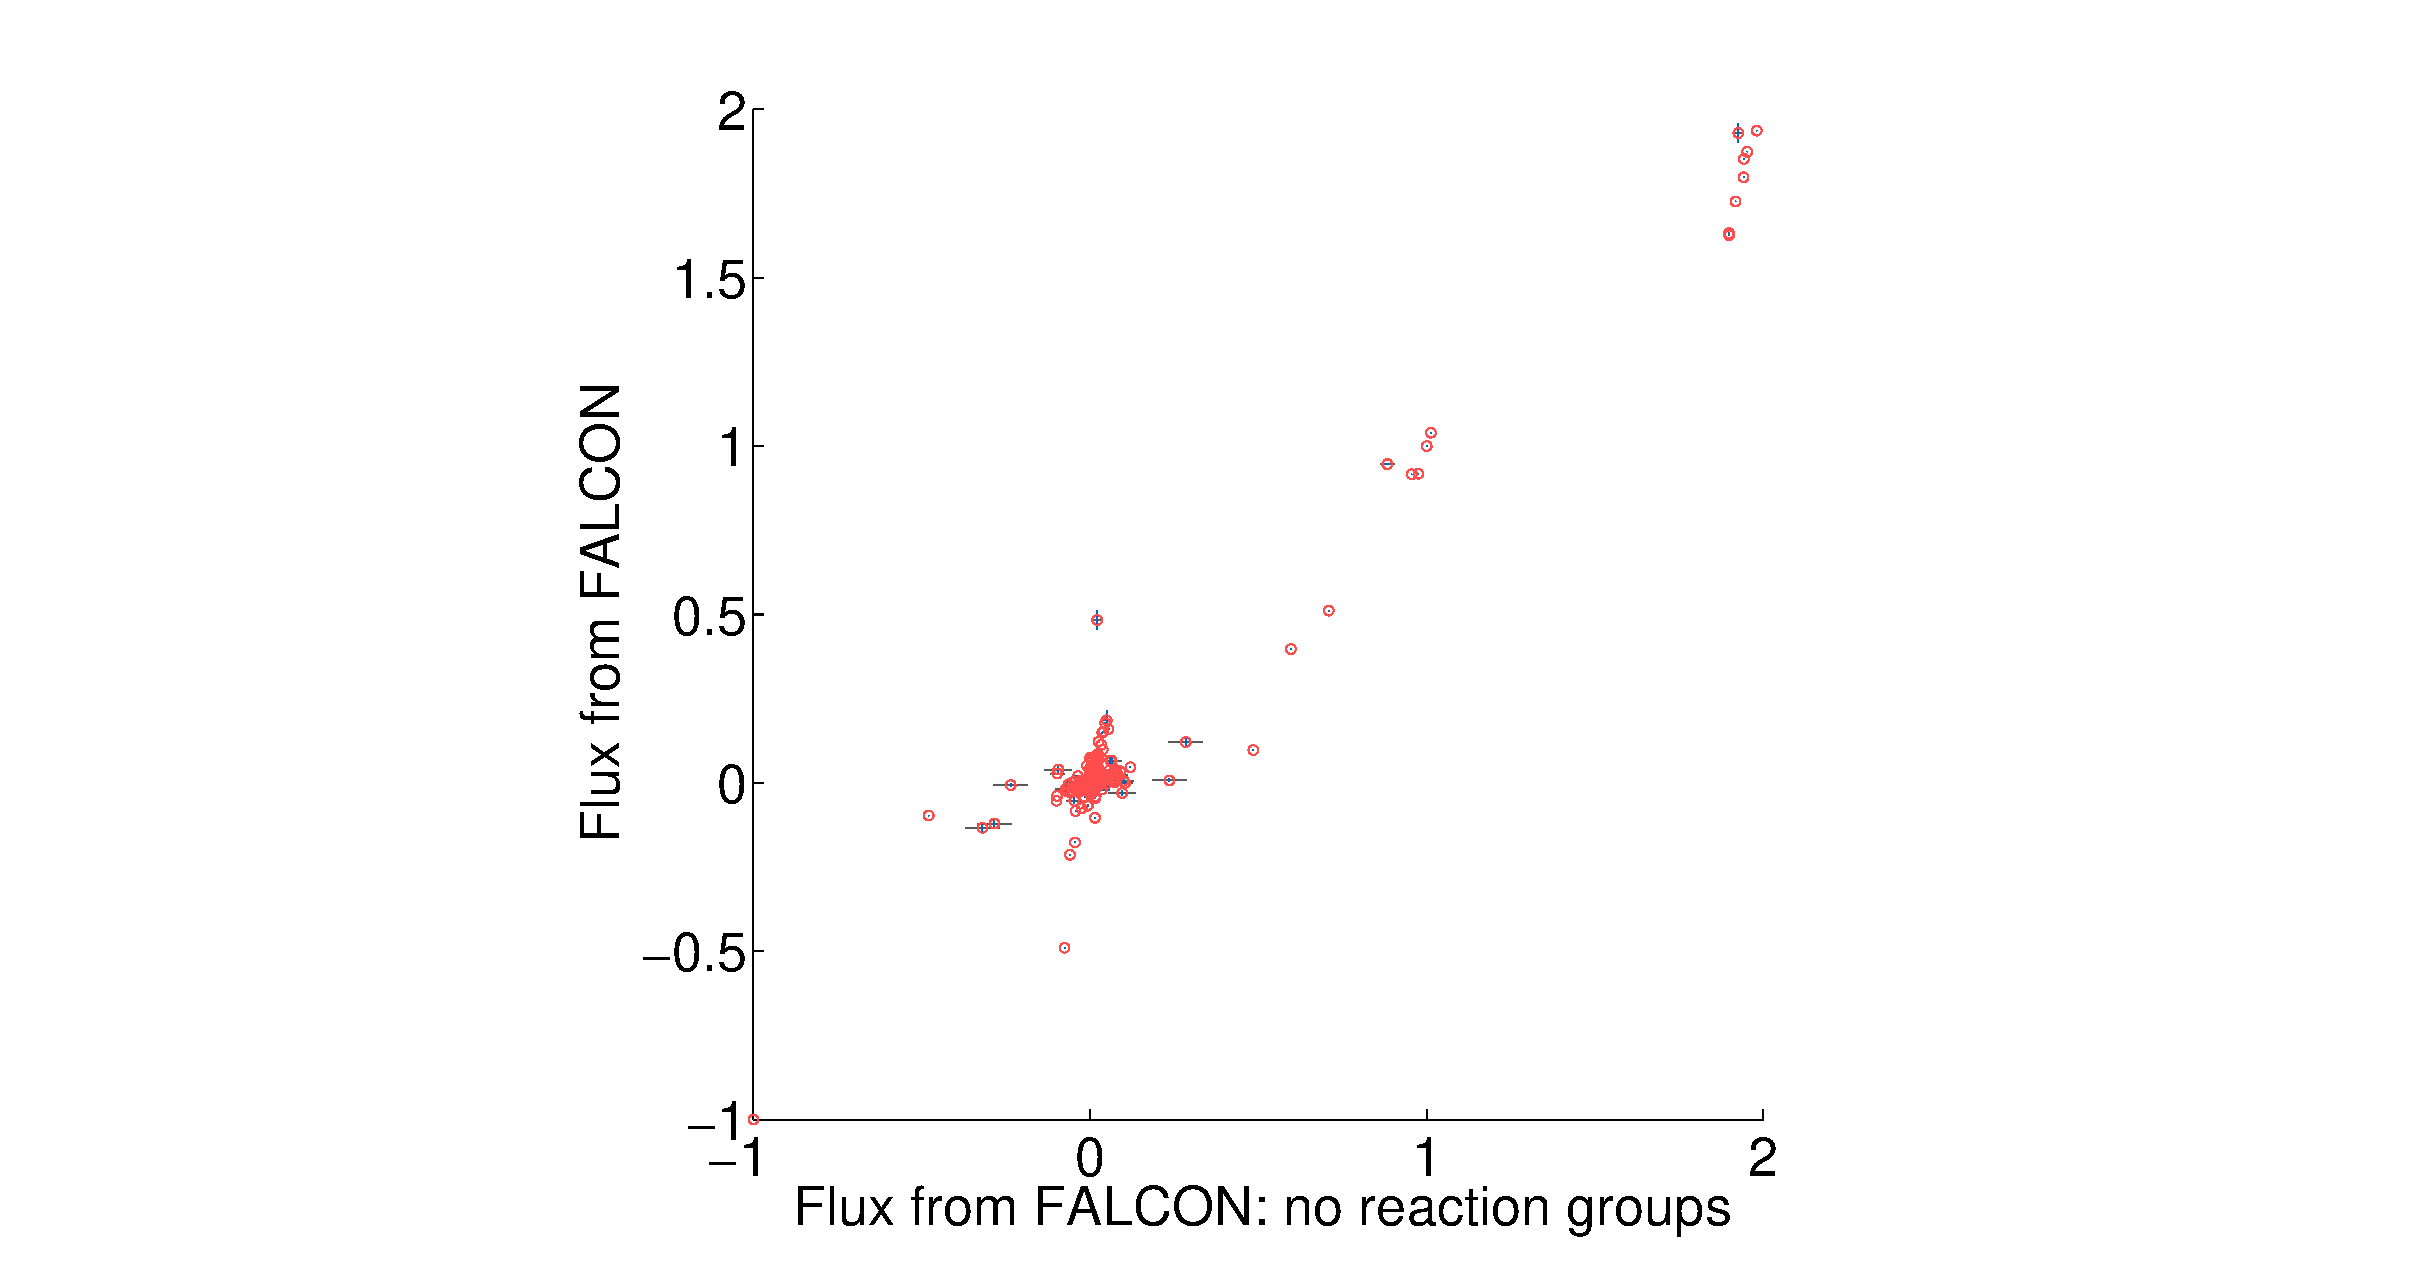
\includegraphics[width=\textwidth, trim=9cm 0cm 9cm 0cm, clip=true]
  {falconGrp_yeastHC}
  \caption{} \label{fig:FalconGrp:A}
  \end{subfigure}
&
  \begin{subfigure}[b]{0.45\textwidth}
  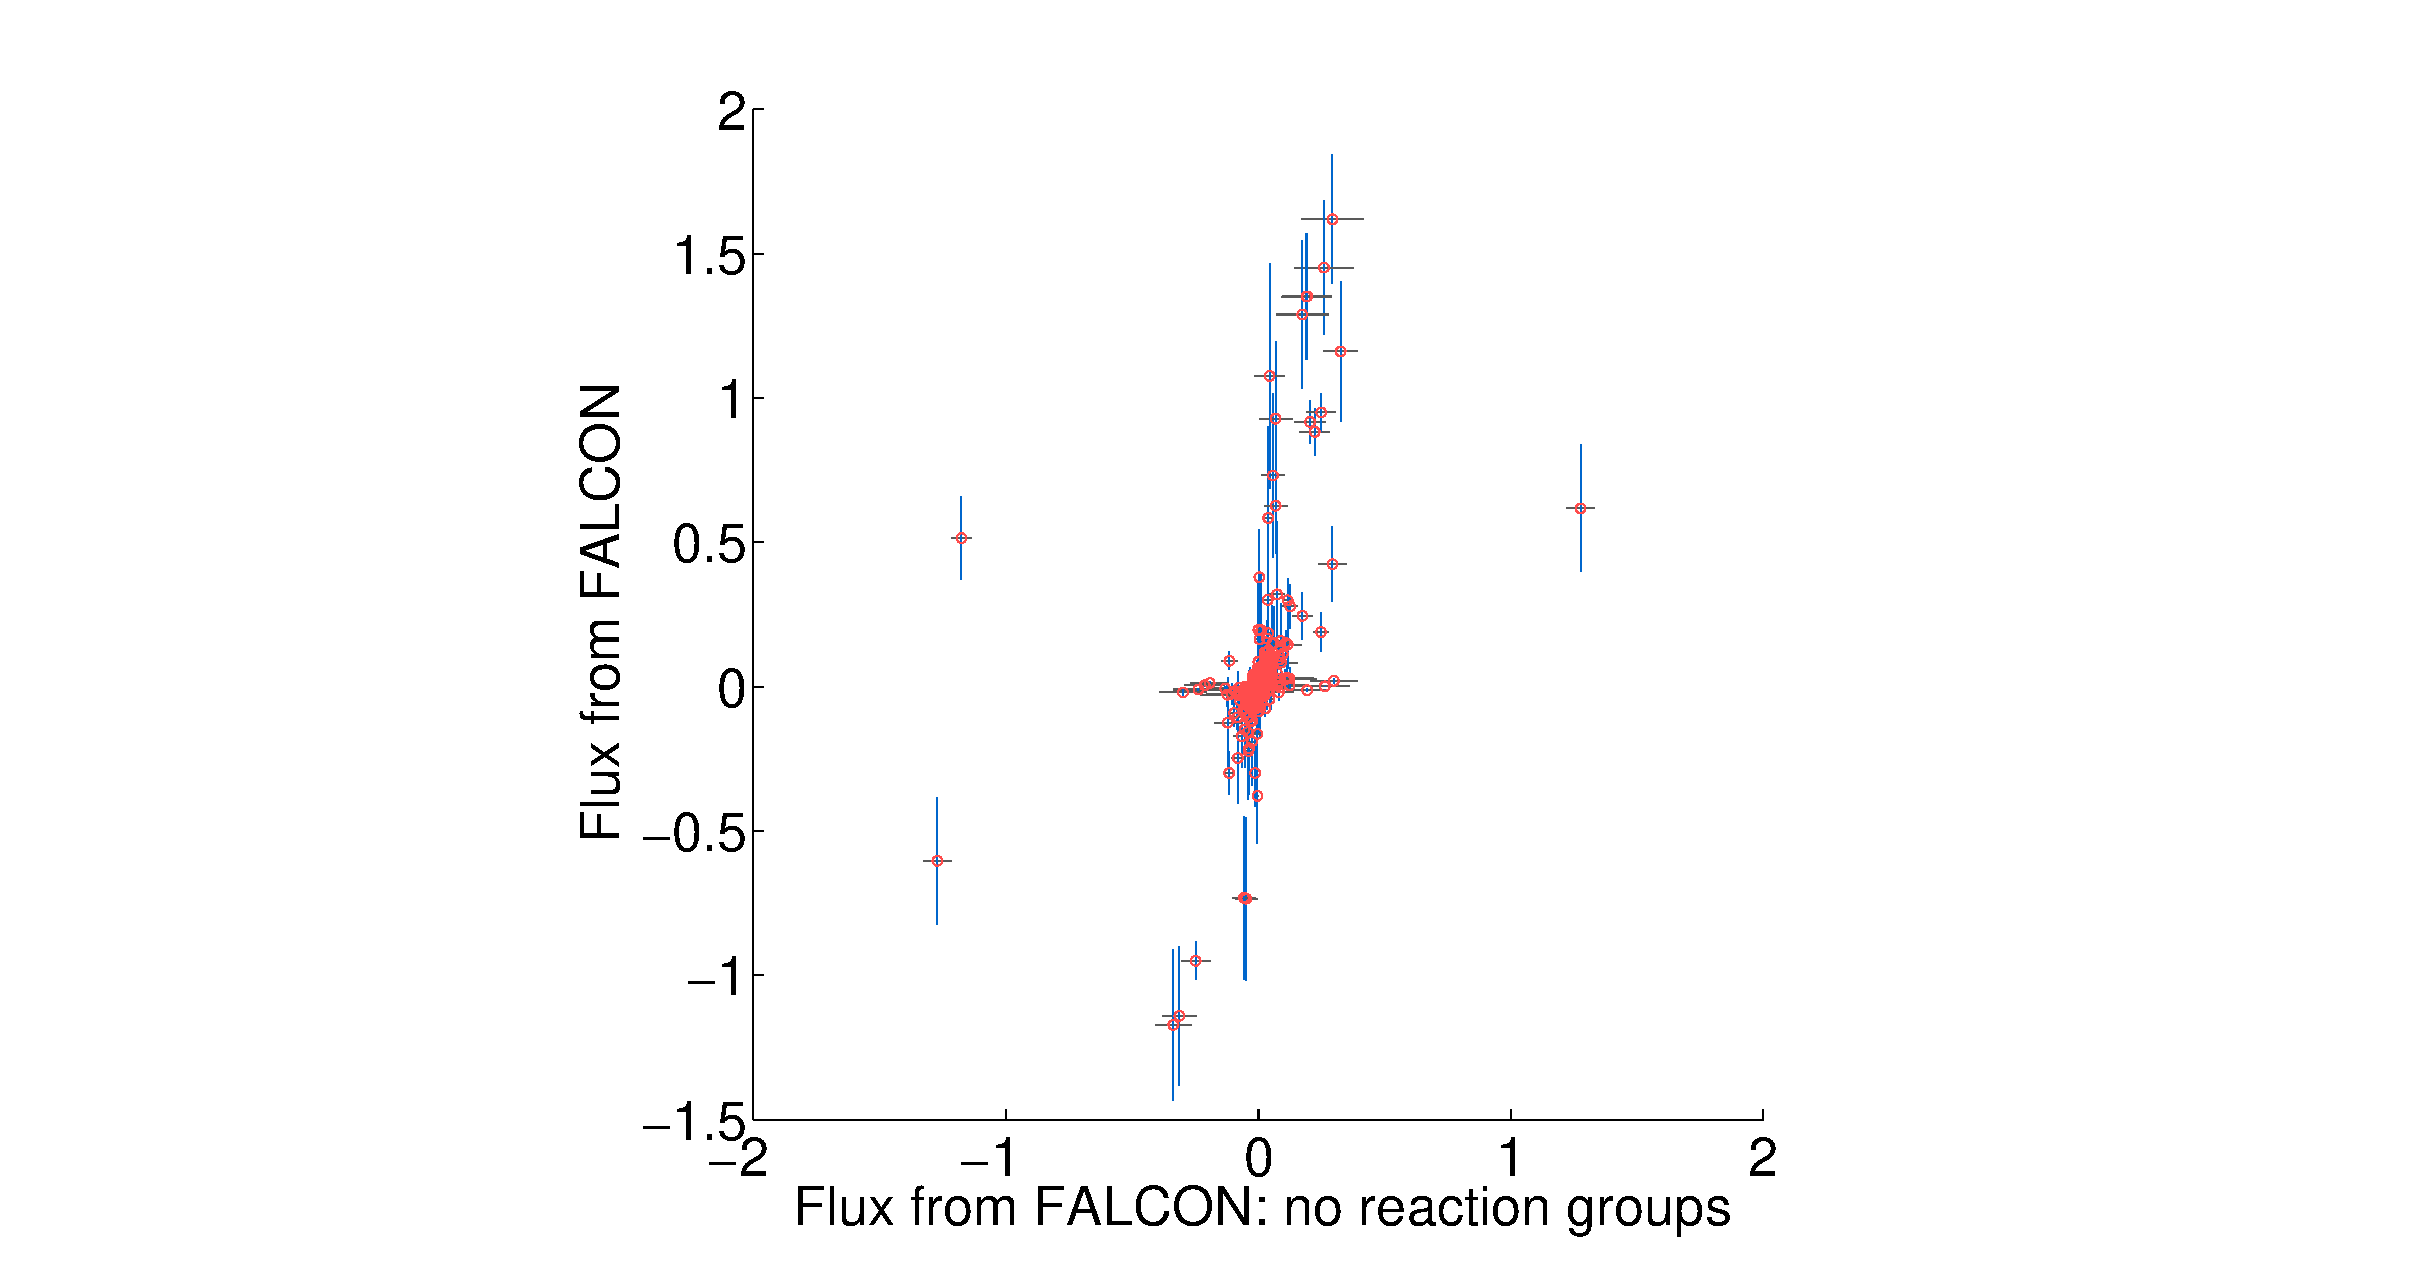
\includegraphics[width=\textwidth, trim=9cm 0cm 9cm 0cm, clip=true]
  {falconGrp_yeastMC}
  \caption{} \label{fig:FalconGrp:B}
  \end{subfigure} 
\\
\end{tabular}
\vspace{-4mm} 
\caption{
Comparison of setting FALCON to use no reaction group information (x-axis)
versus with group information (y-axis; default FALCON setting) with highly  
\textbf{(a)} and minimally \textbf{(b)} constrained models.}
\label{fig:FalconGrp}
\end{figure}
}

%%%%%%%%%%%%%%%%%%%%%%%%%%%%%%%%%%%%%%%%%%%%%%%%%%%%%%%%%%%%%%%%%%%%%%%%%%%%%%%%%%%%%%%%%%


\frame{\frametitle{And, Finally $\dots$} 
\underline{\textsc{Other useful things:}}\\
\footnotesize
\begin{itemize}
	\item Drawing diagrams\\
	\begin{itemize}\footnotesize
		\item[*] \textcolor{darkgreen}{xypic}: draws the diagrams I showed at beginning\\\vspace{.2cm}
		\item[*] the \LaTeX  \hspace{.05cm} \texttt{\textcolor{darkgreen}{picture}} environment \\\vspace{.2cm}
		\item[*] \texttt{\textcolor{darkgreen}{pstricks}}: can't use \textbf{pdflatex} with this\\ \vspace{.2cm}
	\end{itemize}
\item Logo in the footer:\\
\begin{itemize}
	\item[*] put \texttt{$\backslash$\textcolor{Blue}{logo}\{name\}} in preamble\\\vspace{.2cm}
	\item[*] puts logo in bottom right corner\\ \vspace{.2cm}
\end{itemize}
\item References\\
\begin{itemize}
	\item[*] Beamer Users Guide:\\
	 \tiny \url{www.ctan.org/tex-archive/macros/latex/contrib/beamer/doc/beameruserguide.pdf}\\ \vspace{.2cm}\footnotesize
	 \item[*] \footnotesize Google: if you think Beamer should be able to do it, Google it.
\end{itemize}
\end{itemize}
}

%%%%%%%%%%%%%%%%%%%%%%%%%%%%%%%%%%%%%%%%%%%%%%%%%%%%%%%%%%%%%%%%%%%%%%%%%%%%%%%%%%%%%%%%%%
%%%%%%%%%%%%%%%%%%%%%%%%%%%%%% End Your Document %%%%%%%%%%%%%%%%%%%%%%%%%%%%%%%%%%%%%%%%%
%%%%%%%%%%%%%%%%%%%%%%%%%%%%%%%%%%%%%%%%%%%%%%%%%%%%%%%%%%%%%%%%%%%%%%%%%%%%%%%%%%%%%%%%%%

\end{document}

